\documentclass[a4paper,ngerman,12pt]{zirkelblatt1415}

\usepackage[utf8]{inputenc}

\usepackage[ngerman]{babel}

\usepackage{amsmath,amsthm,amssymb,stmaryrd,color,graphicx}
\usepackage{setspace,icomma}
\usepackage{bussproofs}
\usepackage{array}
\usepackage{comment}
\usepackage{graphicx}
\usepackage[protrusion=true,expansion=true]{microtype}

\usepackage{lmodern}

\usepackage{hyperref}

\setlength\parskip{\medskipamount}
\setlength\parindent{0pt}

 \theoremstyle{definition}
 \newtheorem{definition}{Definition}
% \newtheorem{axiom}[defn]{Axiom}
% \newtheorem{bsp}[defn]{Beispiel}

% \theoremstyle{plain}
% \newtheorem{prop}[defn]{Proposition}
% \newtheorem{motto}[defn]{Motto}
% \newtheorem{wunder}[defn]{Wunder}
% \newtheorem{ueberlegung}[defn]{Überlegung}
% \newtheorem{lemma}[defn]{Lemma}
% \newtheorem{kor}[defn]{Korollar}
% \newtheorem{hilfsaussage}[defn]{Hilfsaussage}
 \newtheorem{satz}[definition]{Satz}
% \newtheorem{frage}[defn]{Fragestellung}
 \newtheorem{beispiel}[definition]{Beispiel}
% \newtheorem{problem}[defn]{Problemstellung}


\theoremstyle{remark}
\newtheorem{bem}[definition]{Bemerkung}
% \newtheorem{aufg}[defn]{Aufgabe}

%\newlength{\aufgabenskip}
%\setlength{\aufgabenskip}{1.0em}
%\newcounter{aufgabennummer}
%\newenvironment{aufgabe}[1]{
%  \addtocounter{aufgabennummer}{1}
%  \textbf{Aufgabe \theaufgabennummer.} \emph{#1} \par
%}{\vspace{\aufgabenskip}}

% \clubpenalty=10000
% \widowpenalty=10000
% \displaywidowpenalty=10000

 \setlength\unitlength{1cm}

% \RequirePackage{geometry}
% \geometry{textwidth=16.0cm,textheight=24.5cm,footskip=1.5cm}
% \DeclareGraphicsExtensions{.pdf,.png,.jpg}

\usepackage[bottom=4cm]{geometry}
\usepackage{textcomp}

\newcommand{\RR}{\mathbb{R}}
\newcommand{\CC}{\mathbb{C}}
\newcommand{\ZZ}{\mathbb{Z}}
\renewcommand{\NN}{\mathbb{N}}
\newcommand{\QQ}{\mathbb{Q}}
\newcommand{\lra}{\longrightarrow}
\newcommand{\id}{\text{id}}
\newcommand{\ol}[1]{\overline{#1}}

\begin{document}

\begin{picture}(0,0)
  \put(0,-0.5){%
    \includegraphics[scale=0.1]{bilder/logo-ifm}
  }
  \put(14.0,-3.5){%
    \includegraphics[scale=0.17]{bilder/cover.png}
  }
\end{picture} 

\vspace{6em}


\begin{center}\Large{Vierter Korrespondenzbrief vom \today}\end{center}

\begin{center}\Large{Iterierte Funktionensysteme}\end{center}

In diesem Brief geht es um Funktionen und deren wiederholtes Anwenden. 
In der Schule habt ihr vielleicht bereits Funktionen\footnote{Funktionen werden auch manchmal Abbildungen genannt.} kennengelernt,
hier wollen wir zunächst etwas allgemeiner darüber sprechen. 
Danach schauen wir uns an, was man mit Funktionen so alles anstellen kann, insbesondere betrachten wir die sogenannte Fixpunktiteration.
%und dann Beispiele anschauen, welche "`zeitliche Veränderungen von Zuständen"' 
%beschreiben sollen und so ein "`einfaches"'\footnote{Wie wir sehen werden, sind sie überhaupt nicht einfach.} Beispiel 
%für sogenannte \emph{dynamische Systeme} darstellen.

\section{Grundlagen}

Bevor wir mit Funktionen spielen, wollen wir einige Grundlagen besprechen.
\begin{definition}
Eine \emph{Funktion} $f$ ist eine Abbildungsvorschrift von einer Menge $A$ in eine Menge $B$, kurz $f:A\rightarrow B$, die jedem Element $x$ aus $A$ \emph{genau ein} Element $f(x)$ aus $B$ zuordnet.
Man schreibt auch:
\[
f: x \mapsto f(x). 
\]
$A$ hei{\ss}t \emph{Definitionsbereich} und $B$ \emph{Bildbereich}.
\end{definition}

Was bedeutet das jetzt? Schauen wir uns doch mal ein paar Beispiele an:
\begin{beispiel}
\begin{enumerate}
\item Die Funktion $f$, die zu jeder gegebenen reellen Zahl Eins dazu addiert, ist gegeben durch $f:\RR\lra\RR$ mit $f(x)=x+1$.
\item Die Abbildung "`Verdoppeln"' auf den reellen Zahlen $\mathbb{R}$ kann geschrieben werden als $g:\mathbb{R}\rightarrow\mathbb{R}$ mit
\[
g : x \mapsto 2x
\]
oder kürzer als $g(x)=2x$.
\item Das Runden einer reellen Zahl kann man als eine Funktion $h$ auffassen, $h:\mathbb{R}\longrightarrow\mathbb{Z}$. So gilt zum Beispiel $h(0,321)=0$, $h(0,5)=1$ und $h(2)=2$. 
\end{enumerate}
\end{beispiel}
Solche Funktionen habt ihr vielleicht schon in der Schule gesehen. Aber Funktionen müssen nicht unbedingt auf Zahlen basieren!
Nehmen wir doch mal die Mengen $A = \{ \heartsuit, \diamondsuit, \spadesuit \}$ und $B = \{\clubsuit, \triangle \}$ und die Funktion $h \,:\, A \to B$ mit 
\[ h(x) =\begin{cases} 
      \clubsuit & \text{ für } x = \heartsuit, \\
      \triangle  & \text{ für } x = \diamondsuit, \\
      \clubsuit & \text{ für } x = \spadesuit.  
  \end{cases}
\]
Lustig, nicht? So kann man auch mit Symbolen statt Zahlen rechnen.

Auf jeder Menge $A$ gibt es eine besondere Abbildung, und zwar die Identität $\text{id}_A$, die jedes Element auf sich selbst abbildet. 
Zum Beispiel gilt für $\id_{\RR}\, : \, \RR\lra\RR$, dass $\id_{\RR}(3,7)=3,7$ ist. 
Diese Abbildung hast du vielleicht in der Schule schon kennengelernt, mit dem Funktionsgraphen als ``Winkelhalbierende'', $f(x) = x$.
Wenn nicht, macht das aber auch nichts.

Die Identitätsabbildung darf man aber nicht verwechseln mit einer \emph{konstanten Abbildung} $\text{const}_{c}:\RR\lra\RR$, wobei $c\in\RR$ eine beliebige gewählte (aber jetzt feste) reelle Zahl ist. 
Diese Funktion ist definiert mittels $\text{const}_c(x)=c$, das heißt, sie ordnet \emph{jeder} reellen Zahl die gleiche Zahl zu, nämlich $c$.

Man kann eine Funktion $f$ natürlich dadurch definieren, dass man für jedes Element $x$ das Bildelement $f(x)$ angibt,
so wie ich das für $h$ oben gemacht habe.
Für sehr große Mengen\footnote{Insbesondere gilt dies für unendliche Mengen wie die üblichen Zahlenbereiche $\NN$, $\QQ$, $\ZZ$, $\RR$ und $\CC$.} 
ist das natürlich unpraktisch.
Einfacher ist es, wenn man eine "`Formel"' angibt, welche den Funktionswert durch das Argument ausdrückt. 
Manchmal findet man aber keine einzelne Vorschrift, die für alle Elemente vom Definitionsbereich gilt. 
Betrachte als Beispiel die Betragsfunktion $b:\mathbb{R} \mapsto \mathbb{R}^+_0$, die jeder reellen Zahl eine nichtnegative Zahl zuordnet: 
Jede Zahl $x$, die größer oder gleich Null ist, wird auf sich selbst abgebildet. 
Eine negative Zahl $x$ wird auf $-x$ abgebildet. Man kann also kurz schreiben
\[ b(x) =\begin{cases} 
      x & \text{ für }x\geq 0, \\
      -x & \text{ für }x < 0.
   \end{cases}
\]
Solche Fallunterscheidungen liest man übrigens wie folgt: Wenn das Argument $x$ größer oder gleich Null ist, 
so nimmt $b$ den Wert an, welcher in der Zeile für diesen Fall steht, hier also die obere Zeile, wo $b(x)=x$ notiert ist. 
Falls aber $x<0$ gilt, so sind wir auf der unteren Zeile, wo $b(x)=-x$ steht.
Für den Betrag einer Zahl $x$ schreibt man üblicherweise $|x|$ weil man keine Lust hat, das so kompliziert zu machen,
also gilt $b(x)=|x|$. 
Man bekommt also beispielsweise $b(3,7) = |3,7| = 3,7, b(-5) = 5$ und $b(100-3) = 97$ heraus.


Als weiteres Beispiel können wir eine Funktion $r$ definieren, die jeder natürlichen Zahl ihren Rest bei der Division durch $2$ zuordnet: $r:\mathbb{N}_0 \longrightarrow \{0\text{, }1\}$ mit
\[ r(a) = 
\begin{cases}
0 & \text{ wenn }2\mid a, \\
1 & \text{ wenn }2\nmid a.
\end{cases}
\]
Hier bedeutet $2 \mid a$, dass $2$ ein Teiler von $a$ ist, also $a$ gerade ist, und $2\nmid a$ genau das Gegenteil. 

\begin{aufgabe}{Werten wir das doch mal aus! -- eine Miniaufgabe}
 Hier kannst du mal ein paar Funktionen auswerten:
 Bestimme $r(3), r(5), h(\heartsuit), b(-5)$!
 Wenn du schon Funktionen kennst, verrrate mir doch deine momentane Lieblingsfunktion!
\end{aufgabe}

Wir sagen, dass es sich in den Fällen von $b$ und $r$ um \emph{abschnittsweise definierte Funktionen} handelt.
Abschnittsweise deshalb, weil man verschiedene Fälle haben kann. Bei $f(x) = 2x$ muss man dagegen nicht darauf achten, was man einsetzt -- 
es gibt keine Fälle zu beachten.

Da wir uns jetzt ein paar Beispiele von Funktionen angesehen haben, 
können wir ein wenig mutiger werden und versuchen, Funktionen zu erforschen.
Dazu werde ich euch jetzt zwei Begriffe zeigen, vor denen meine Studentinnen und Studenten manchmal am Anfang Angst haben. 
Dabei ist das alles gar nicht schlimm.
Hier kommen sie: \emph{injektiv} und \emph{surjektiv}!
Was heißt das jetzt genau?

Gucken wir uns mal die Funktion $z \,:\, A \to B$ an, wobei 
$A = \{ \text{Julia}, \text{Sandra}, \text{Martin}\}, B = \{\text{Bonbon}, \text{kein Bonbon} \}$ mit 
\[ z(x) =\begin{cases} 
      \text{Bonbon} & \text{ für } x = \text{Julia}, \\
      \text{kein Bonbon}  & \text{ für } x = \text{Sandra}, \\
      \text{Bonbon} & \text{ für } x = \text{Martin}.  
  \end{cases}
\]
Eine Funktion heißt surjektiv, wenn ihr ganzer Bildbereich "`getroffen"' wird. 
Die Funktion~$z$ ist surjektiv, da man sowohl \emph{Bonbon}, als auch \emph{kein Bonbon} als Wert bekommt.
Wenn man $z$ ändert zu $z(x) = \text{kein Bonbon für alle $x$ aus }A$, ist sie nicht mehr surjektiv,
da der Wert \emph{Bonbon} mit keinem der Werte aus $A$ getroffen wird. 
(Ziemlich traurig, dieser Fall, da jetzt keines der Kinder mehr Bonbons erhält\ldots Der fröhlichere Fall 
 $z(x) = \text{Bonbon für alle $x$ aus }A$ ist aber auch nicht surjektiv).

Die Funktion $z$ wie zu Beginn beschrieben ist aber nicht injektiv. Injektiv bedeutet, dass zu jedem Fall im Bild, also zu 
Bonbon und nicht Bonbon nur ein einziges Kind (oder keines) existiert, welches diesen Fall auslöst. 
Das stimmt aber nicht. Sowohl Julia und Martin lösen beide das Bonbon aus.

\begin{aufgabe}{Injektiv?}
 Kann man $z$ irgendwie so verändern, dass es injektiv wird? Warum nicht? 
\end{aufgabe}

Gucken wir uns noch $f \, : \, \mathbb{R} \to \mathbb{R}$ mit $f(x) = x^2$ an.
Hier wirst du gleich feststellen, dass es ganz wichtig ist, welche Mengen $A$ und $B$ man bei so einer Funktion hinschreibt.
Ist $f$ denn surjektiv? Dazu müssen wir uns anschauen ob ganz $\mathbb{R}$ "`getroffen"' wird.
Das ist aber leider nicht der Fall, weil man zum Beispiel $-4$ nie als Ergebnis von $f$ herausbekommen wird, egal was man einsetzt\footnote{ Auch $f(-2)$ ist $+4$, nicht $-4$!}.
Injektiv ist sie auch nicht, denn $3$ und $-3$ führen beide zum gleichen Wert $f(-3) = 9 = f(3)$.

Wenn man die Funktion ein bisschen anders definiert, klappt es aber.
Wir streichen einfach die negativen Zahlen weg und arbeiten mit $\mathbb{R}^+_0$ statt $ \mathbb{R}$,
$f \, : \, \mathbb{R}^+_0 \to \mathbb{R}^+_0$ mit $f(x) = x^2$ ist sowohl injektiv als auch surjektiv.
Dabei sind in $\mathbb{R}^+_0$ alle positiven reellen Zahlen enthalten, sowie die $0$.
Das mathematisch sauber zu beweisen ist übrigens nicht schwer, nur etwas technisch und es erfordert etwas höhreres Schulwissen, das können 
wir also getrost meinen Studentinnen und Studenten überlassen.

Abbildung \ref{abbb1} auf der Rückseite zeigt noch mehr Beispiele. Was die jeweilige Funktion mit den Elementen der Menge macht, habe ich mit den Pfeilen dargestellt.
Die Funktion links oben ist surjektiv, denn alle Werte aus $B$ werden getroffen. Injektiv ist sie nicht, denn $f(1) = f(7)$.
Die Funktion rechts oben ist injektiv, denn kein Wert in $B$ wird von mehr als einem Element in $A$ "`getroffen"', 
aber da $5$ nicht getroffen wird, ist sie nicht surjektiv.
Links unten ist ein Beispiel einer Funktion, die weder surjektiv noch injektiv ist. 
Wieder wird $5$ nicht getroffen, und $f(1) = f(7)$.
Rechts unten ist die Funktion dagegen sowohl surjektiv als auch injektiv.

\begin{figure}
\begin{center}
 \hspace*{-1cm}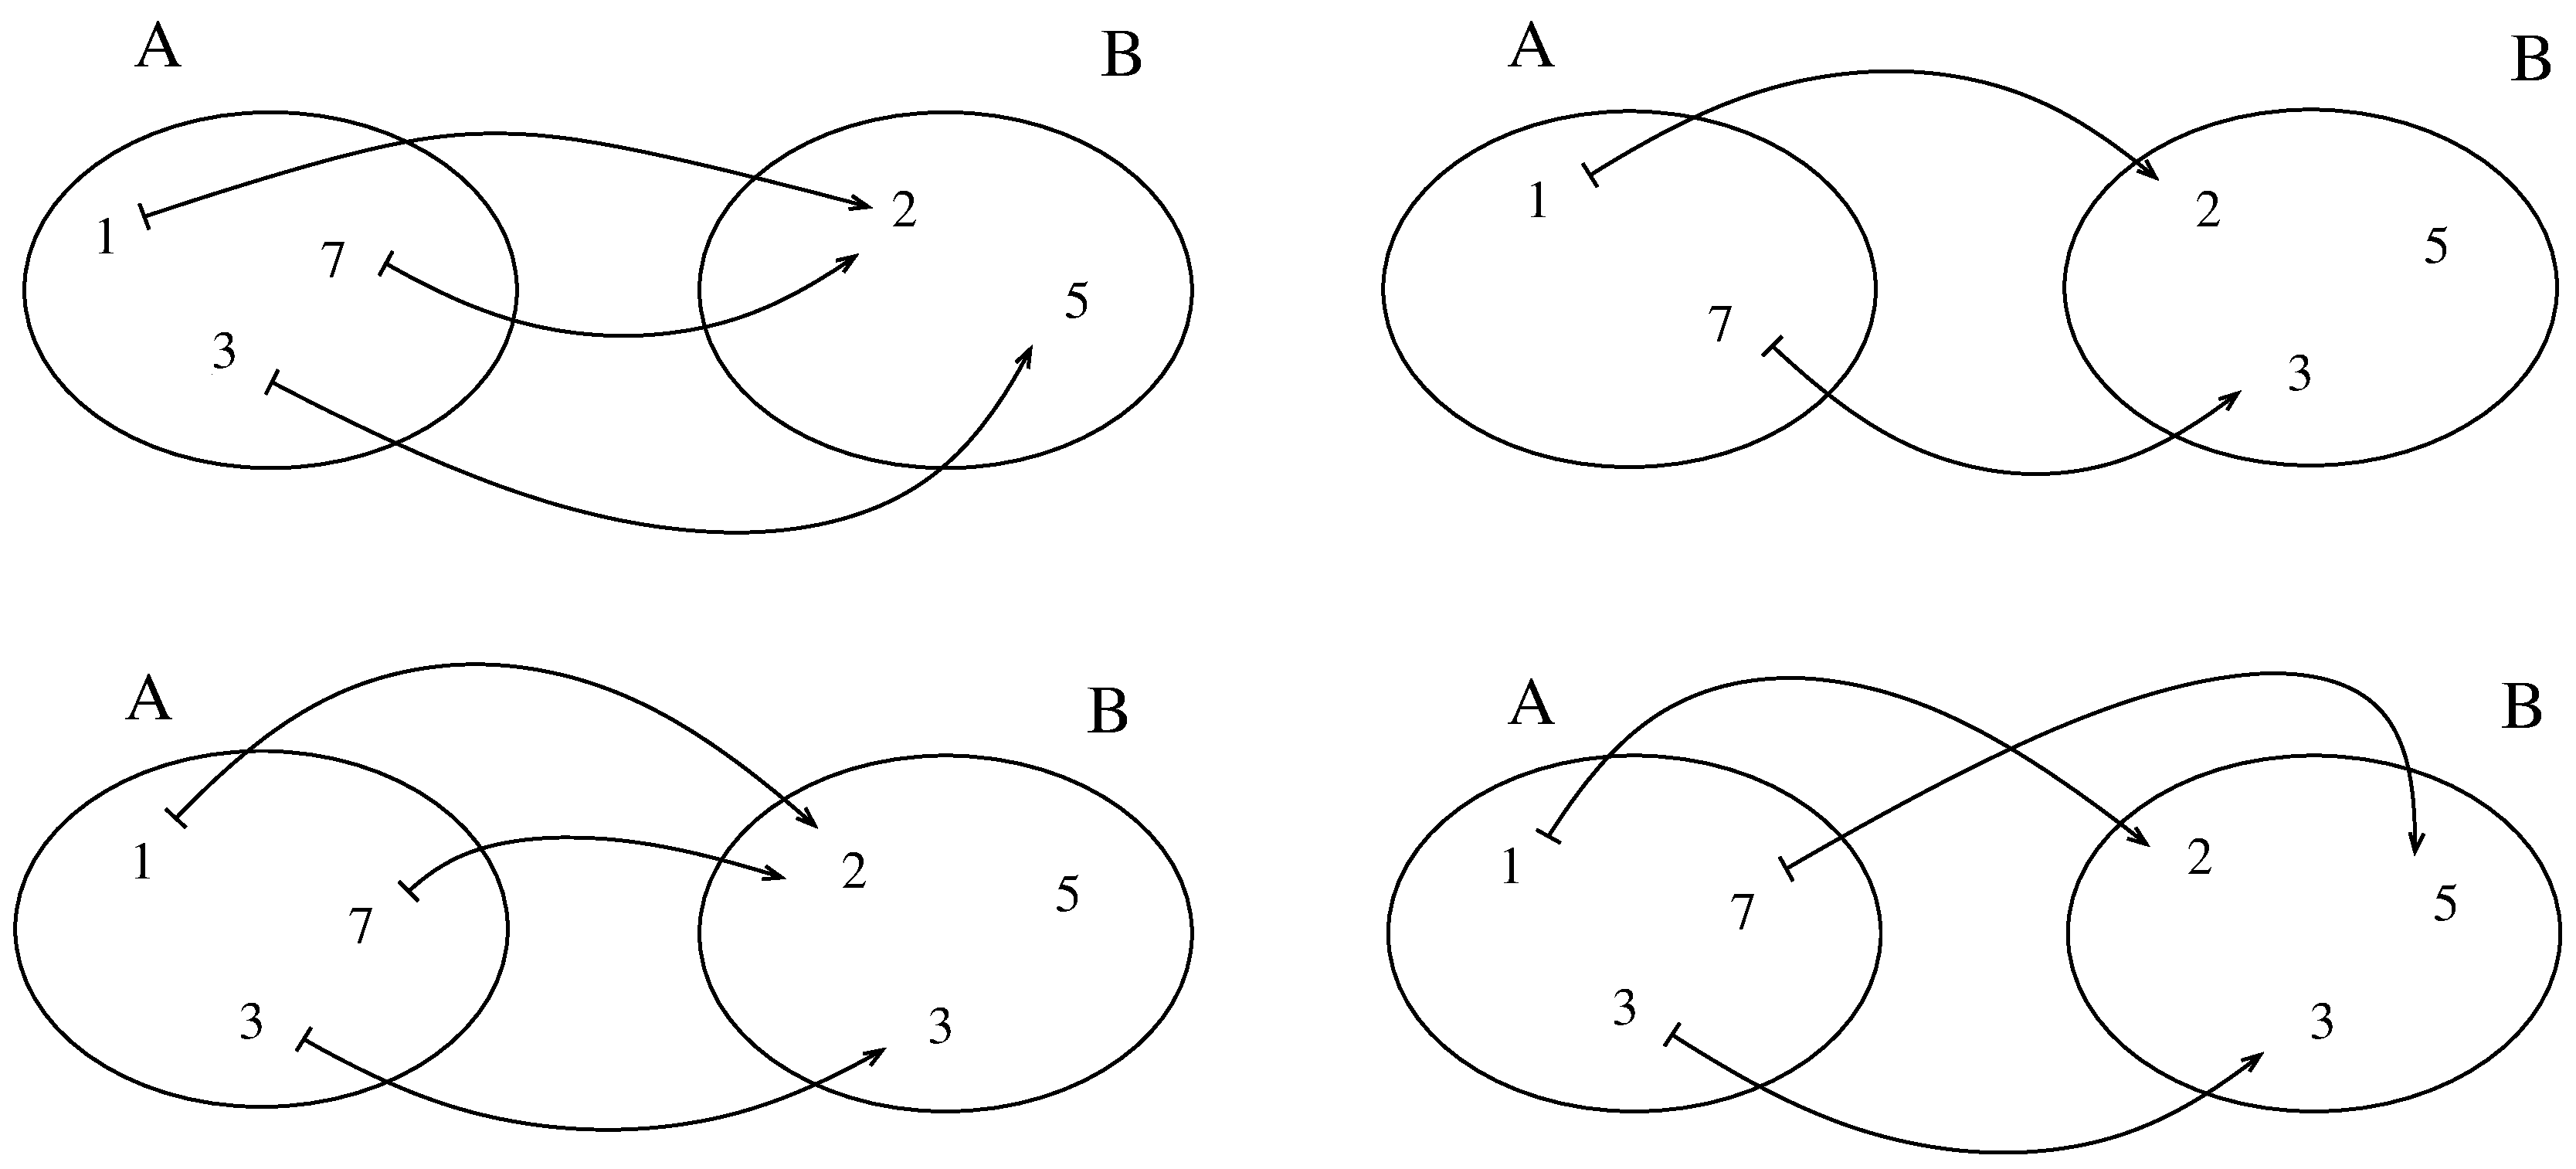
\includegraphics[scale = 0.3]{bilder/abb1}
 \caption{Vier verschiedene Abbildungen zwischen unterschiedlichen Mengen.} \label{abbb1}
\end{center}
\end{figure}


\begin{aufgabe}{Surjektiv und Injektiv}
 Jetzt darfst du dir mal ein paar Funktionen angucken und die überlegen, ob sie surjektiv und injektiv sind.
 Hier sind meine Beispiele:
 \begin{itemize}
  \item Die Funktion $z \,:\, A \to B$, wobei 
        $A = \{ \text{Huhn}, \text{Kuh}, \text{Schaf}\}, B = \{\text{Ei}, \text{Milch}, \text{Wolle} \}$ mit 
        \[ z(x) =\begin{cases} 
             \text{Ei} & \text{ für } x = \text{Huhn},\\
              \text{Milch}  & \text{ für } x = \text{Kuh},\\
              \text{Wolle} & \text{ für } x = \text{Schaf}.  
               \end{cases}
         \]
   \item Die Funktion $b \, : \, \mathbb{R} \to \mathbb{R}$ mit $b(x) = | x |$.   
   \item Die Funktion $r \, : \, \mathbb{N} \to \mathbb{N}$
         \[ r(a) = 
         \begin{cases}
          0 & \text{ wenn }2\mid a, \\
          1 & \text{ wenn }2\nmid a.
          \end{cases}
           \]
 \end{itemize}
 Wie kann man bei $r$ den Wertebereiche ändern, um sie surjektiv zu machen?
 Ist deine Lieblingsfunktion surjektiv und injektiv? Wenn das zu schwierig ist, darfst du sie mir gerne verraten, 
 dann kann ich dir die Antwort darauf geben. 
\end{aufgabe}

Warum ist das Ganze so spannend?
Wenn eine Funktion sowohl surjektiv, als auch injektiv ist, ist sie \emph{umkehrbar}.
Man kann ihre Anwednung sozusagen rückgängig machen. Das ist oft sehr praktisch, daher sind solche Funktionen sehr beliebt.
Zuerst müssen wir uns dazu allerdings anschauen, wie man zwei Funktionen verknüpft.

Wenn wir zwei Abbildungen $f$ und $g$ haben, 
können wir beide unter bestimmten Voraussetzungen \emph{miteinander verknüpfen} und so eine neue Funktion erhalten.
\begin{definition}
Seien $f: A\longrightarrow B$ und $g: B\longrightarrow C$ zwei Abbildungen. Dann ist die Verknüpfung $g\circ f$ (ausgesprochen "`$g$ nach $f$"') eine Abbildung von $A$ nach $C$, die definiert ist als
\[
g\circ f: x \mapsto g\left(f(x)\right)
\]
oder anders geschrieben
\begin{equation*}
  (g\circ f)(x)=g(f(x)),
\end{equation*}
das heißt, zuerst wendet man $f$ an und danach $g$ auf das Ergebnis von $f$.
\end{definition}

\begin{bem}
  Beachte, dass die Reihenfolge der Schreibweise ziemlich komisch ist: $g\circ f$ bedeutet, dass $f$ zuerst angewendet wird und nicht $g$. 
  Das bedeutet, dass man praktisch von innen nach außen vorgeht. 
  Das verknüpfte Abbildung nennt man auch manchmal die \emph{Komposition}.
\end{bem}

\begin{beispiel}
  \begin{enumerate}
    \item 
    Sei $f:x\mapsto 2x$ und $g:x \mapsto x^2$. Dann ist
      \[
        g\circ f: x\mapsto (2x)^2 = 4x^2.
      \]
    \item Sei jetzt $f:x \mapsto x-3$ und $g:x \mapsto x^2 +1$. Dann ist 
    \[
        g\circ f: x\mapsto (x-3)^2 +1.
      \]
      Achtung: $g \circ f$ ist \underline{nicht} $x \mapsto x-3^2 +1$.
      Man muss den Funktionsausdruck $x-3$ nämlich wie eine Zahl in $g$ 
      einsetzen und dadurch wird der ganze Ausdruck quadriert.
 \end{enumerate}
\end{beispiel}

\begin{aufgabe}{Vertauschen von Kompositionen}
Im Allgemeinen, selbst wenn $f:A\mapsto A$ und $g:A\mapsto A$, haben wir
\[
f\circ g \neq g \circ f,
\]
man kann also die Reihenfolge der Funktionen nicht generell vertauschen. 
Probiere doch mal zwei Funktionen $f$ und $g$ zu finden, so dass $f\circ g$ und $g\circ f$ einen Unterschied macht.

\textbf{Tipp (falls du nicht weiter kommst):} Wir haben uns oben ja schon ein paar Funktionen angeschaut, und aus der Schule kennst du vielleicht auch schon viele.
Nimm dir einfach zwei her, und such dir einen beliebigen Wert $x$ aus, zum Beispiel $x=3$.
Und jetzt guckst du, ob $f(g(3)) = g(f(3))$ gilt. Wenn nicht, hast du dein Gegenbeispiel gefunden, prima!
\end{aufgabe}

Eine interessante Frage ist, ob man eine gegebene Abbildung ``umkehren'' kann, also rückgängig machen kann.
Das hatten wir uns ja auf der vorigen Seite schon gefragt. 
Schauen wir uns doch mal die folgende Definition an:
\begin{definition}
Sei $f:A\longrightarrow B$. Eine Abbildung $f^{-1}:B\longrightarrow A$ heißt \emph{Umkehrabbildung} von $f$, wenn gilt:
\begin{align*}
f\circ f^{-1}& = \text{id}_B\\
f^{-1}\circ f& = \text{id}_A.
\end{align*}
\end{definition}

Was soll das nun bedeuten? Wirf mal einen Blick auf den Definitions- und Wertebereich der Umkehrfunktion $f^{-1}$.
Das ist genau anders herum als bei $f$ -- logo --  man will ja auch $f$ sozusagen rückgängig machen.
Der Rest der Definition ist ebenfalls einfach zu erklären:
Die Gleichheit $f\circ f^{-1} = \text{id}_B$ bedeutet nämlich einfach, dass ich mir jeden Punkt $x$ aus $B$ hernehmen kann 
und dass dann immer gilt $f ( f^{-1}(x)) = x$.
Anders herum bedeutet $f^{-1}\circ f = \text{id}_A$, dass man immer $f^{-1} ( f(y)) = y$ hat, egal welches $y$ aus $A$ man in diese 
Verkettung einsetzt.
Genau so ein Verhalten will man haben, wenn man eine Umkehrabbildung sucht.
Wenn du noch mal einen Blick auf Abbildung \ref{abbb1} wirfst, siehst du, dass man die Abbildung rechts unten umkehren kann.
Bei der Umkehrabbildung muss man einfach nur die Pfeile anders herum einzeichnen und dann ist die obige Definition erfüllt.

\begin{aufgabe}{Warum geht es bei den anderen nicht?}
Überlege dir doch mal, warum es bei den anderen drei Abbildungen nicht klappt!
\end{aufgabe}
% Die Funktionen hier und aus der Schule sind meistens Abbildungsvorschriften, in die man Zahlen aus z.B. $\mathbb{R}$ einsetzen kann.
% Man kann also unendlich viele Werte einsetzen.
% Jetzt gibt es aber auch die Möglichkeit Funktionen auf endlichen Mengen anzuschauen. Das mag einem viel langweiliger erscheinen,
% aber tatsächlich sind endliche Mengen recht spannend, die \emph{Algebra} beschäftigt sich ganz gerne damit.
% 
% \begin{aufgabe}{Endliche Mengen und Abbildungen}
% Seien $A$ und $B$ endliche Mengen und $f:A\longrightarrow B$ eine Abbildung zwischen diesen.
% Zum Beispiel könnte $A = \{ 1, 2, 3 \}$ sein und $B = \{ 0, 5\}$.
% Und $f$ könnte vielleicht so aussehen: $f(1) = 0, f(2) = 0, f(3) = 5$.
% Das wäre jetzt mal so ein Beispiel einer Abbildung $f$ zwischen zwei endlichen Mengen. Eigentlich einfach, oder?
% 
% Beweise die folgende Aussage:
% 
% Wenn $A$ und $B$ unterschiedlich viele Elemente haben, kann es keine Umkehrabbildung $f^{-1}$ zu $f$ geben.
% 
% Tipp: Behandle die beiden Fälle
% \begin{enumerate}
% \item $A$ hat mehr Elemente als $B$ und
% \item $B$ hat mehr Elemente als $A$
% \end{enumerate}
% einzeln.
% \end{aufgabe}

% \begin{aufgabe}
% Beweise die folgende Aussage: 

% Erfüllt die Funktion $f:A\longrightarrow B$ die beiden Eigenschaften:
% \begin{itemize}
% \item $f$ ist injektiv: Es gibt keine zwei verschiedenen Elemente $x_1$ und $x_2$ mit $f(x_1)=f(x_2)$.
% \item $f$ ist surjektiv: Jedes Element $y$ von $B$ ist Bild eines Element von $A$.
% \end{itemize}
% \end{aufgabe}





\section{Iterierte Funktionsysteme}

Haben wir eine Funktion $f:A\longrightarrow A$ von einer Menge in sicher selber, können wir diese immer wieder mit sich selbst verknüpfen. 
Dies bezeichnen wir als iteriertes\footnote{Iterieren bedeutet einfach Wiederholen.} Funktionsystem $f$ auf $A$.

\begin{beispiel}
\label{bsp11}
Wir haben die Menge $A=\{1,2,3,4 \}$. Betrachte die Funktion
\begin{align}
f(x)=\begin{cases}
2 & x=2, \\
4 & x=1 \text{ oder }x=3, \\
3 & x=4.
\end{cases} \label{beispiel}
\end{align}
%Das wird unsere Standardbeispiel für den Rest dieses Abschnitts. 
\end{beispiel}



\begin{aufgabe}{Funktionsgraphen}
  In der Schule lernt ihr das auch sehr intensiv kennen: Malt den \emph{Funktionsgraphen} von $f$. 
  Das heißt, ihr tragt in der horizontalen Richtung die $x$-Werte zum Beispiel von $-4$ bis $4$ und in der vertikalen Richtung die zugehörigen Werte von $f(x)$ ab. 
  Dies hilft um sich vorzustellen, was eine Funktion macht.
\end{aufgabe}

Da es sehr mühsam ist, mit $\circ$ die Verknüpfung zu schreiben, wenn man eine Funktion ganz oft mit sich selbst verknüpft, 
gibt es eine verkürzende Schreibweise.

\begin{definition}
Wir definieren
\begin{align*}
f^n &:= \underbrace{f \circ f \circ f \circ \ldots \circ f}_{\text{n Mal}}, \\
f^0 &:= \id_A.
\end{align*} 
\end{definition}
Was bedeutet diese Definition anders erklärt? $f^0$ bedeutet, dass wir die Funktion $0$ Mal, also gar nicht, auf einen Wert $x$ anwenden.
Das ist das gleiche, wie die Identitätsfunktion auf $x$ anzuwenden, denn -- wir erinnern uns -- die lässt den Wert ja unverändert.
Und~$f^n$? Das bedeutet einfach, dass man die Funktion $n$ mal auf einen Wert anwendet. Also für $n = 4$ 
ist $f^4 (x) = f(f(f(f(x))))$. (Jetzt merkst du bestimmt, warum man lieber die kürzere Schreibweise nimmt.)

\begin{beispiel}
 Nehmen wir doch die Funktion $f$ aus Beispiel \ref{bsp11} her.
 Was ist dann $f^4(1)$? Da $f(1) = 4$, ist $f^2(1) = f(f(1)) = f(4) = 3$, also ist $f^3(1) = f(f(f(1))) = f(f^2(1)) = f(3) = 4$.
 Und damit gilt dann $f^4(1) = f(f^3(1)) = f(4) = 3$.
\end{beispiel}


Wozu wollen wir nun überhaupt solche iterierten Funktionen anschauen? 
Eine mögliche Interpretation ist die folgende: 
Stellt euch vor eure Menge $A$ beschreibt gewissen Zustände in welchem sich ein physikalisches System befinden kann. 
Zum Beispiel könnte $A=\{\text{Kopf, Zahl}\}$ die Zustände einer Münze beschreiben. 
Dann könnte $f:A\lra A$ eine (festgelegte) Änderung dieses Zustands beschreiben und die Anwendung von $f$ entspricht einem "`Zeitschritt"' oder einer solchen Änderung. 
Beispielsweise würde
\begin{equation*}
  f(x)=\begin{cases} \text{Kopf} \quad \text{ für } x=\text{Zahl},\\ \text{Zahl} \quad \text{ für }x=\text{Kopf},\end{cases}
\end{equation*}
dem einmaligen Umdrehen der Münze entsprechen. Das heißt, $f^n$ beschreibt das $n$-malige Umdrehen der Münze.

Bei einem iterierten Funktionensystem interessiert man sich vor allem, wie sich ein Punkt $x$ verhält, wenn wir die Abbildung sehr oft anwenden. 
Dazu gibt es den Begriff des Orbits.

\begin{definition}
Sei $x$ ein Punkt aus $A$. Der Orbit\footnote{Orbit heißt Laufbahn. Die Bezeichnung kommt daher, dass man sich vorstellt, 
dass $x$ eine Position eines Punktes ist, der sich nach folgender Regel bewegt: 
Ist der Punkt zu einem Zeitschritt am Ort $x$, ist er im nächsten Zeitschritt am Ort $f(x)$.} 
von $x$ unter $A$ ist die Menge
\[
\mathcal{O}^+(x) = \{x, f(x), f^2(x), f^3(x) ,\ldots\}.
\]
Der Orbit scheint also zunächst unendlich zu sein, denn es geht immer weiter... 
\end{definition}


\begin{beispiel}
Nehmen wir doch mal den Punkt $1$ her.
Mit dem System aus Beispiel \ref{bsp11} ist $\mathcal{O}^+(1) = \{1,4,3,4,3,\ldots\}$.
Wie geht das denn weiter?
\end{beispiel}



\begin{aufgabe}{Orbit einer Abbildung}
  So, jetzt darfst du das mal versuchen! 
  \begin{enumerate}
    \item Bestimme den Orbit von $2$ unter $f$ aus Beispiel~\ref{bsp11}.
    \item Bestimme den Orbit von $3$ unter $f$ aus Beispiel~\ref{bsp11}.
  \end{enumerate}
\end{aufgabe}

% Bis hierher grob durchgesehen, Sven.

Das einfachste Verhalten ist natürlich, wenn der Orbit nur aus einem Punkt besteht.
In diesem Fall hat der Punkt einen besonderen Namen.
\begin{definition}
Ein Punkt $x^{*}$ heißt Fixpunkt, wenn gilt $f(x^{*}) =x^{*}$.
\end{definition}

Fixpunkte sind bei Mathematikerinnen und Mathematikern sehr beliebt, weil sie einfach schön sind.
Darum nennen Mathematiker sie auch fast immer $x^{*}$, weil Sternchen auch so schön sind.

Manchmal kann man sie ganz leicht ausrechnen.
\begin{beispiel}
  Gucken wir uns doch mal $f \, : \, \mathbb{R} \to \mathbb{R}$ an, mit $f(x) = x^2 + 3x$.
  Ein Fixpunkt ist Lösung der Gleichung $f(x) = x$, also $x^2 + 3x = x$.
  Und das kann man ziemlich leicht lösen, denn wir subtrahieren einfach $x$ und bekommen $x^2 + 2x = 0$.
  Jetzt kann man ein $x$ ausklammern und wir haben $x (x + 2) = 0$. Als Lösung kommt also $x^{*} = 0$ oder 
  $x^{*} = -2$ infrage. 
\end{beispiel}

\begin{aufgabe}{Fixpunkte -- sie sind einfach überall!}
  Bestimme die Fixpunkte der Funktionen 
  \begin{itemize}
   \item $f \, : \, \mathbb{R} \to \mathbb{R}$ an, mit $f(x) =  x^3 - 3x$,
   \item $f \, : \, \mathbb{R} \to \mathbb{R}$ an, mit $f(x) = -x^2 + 1$.
  \end{itemize}
  Ein Fixpunkt der letzten Funktion ist übrigens der goldene Schnitt! 
  Wenn du den nicht kennst, ist das gar nicht schlimm, aber es ist schon erstaunlich, was sich so alles als Fixpunkt entpuppen kann, nicht wahr?
\end{aufgabe}

Manchmal lässt sich ein Fixpunkt nicht so einfach ausrechnen, weil es sehr komplizierte Funktionen gibt.
Aber man kann ihn manchmal trotzdem mit dem Taschenrechner annähern, was ich dir jetzt zeigen werde.
Wenn man eine Funktion $f$ hat und man möchte das Fixpunktproblem $f(x) = x$ näherungsweise lösen, geht man wie folgt vor:
Man nimmt einen beliebigen Wert $x_0$ als Startwert. Am besten ist es, wenn der Wert in der Nähe des vermuteten Fixpunktes liegt,
aber das ist im Allgemeinen natürlich schwierig, weil man den Fixpunkt nicht kennt.
Und jetzt wendet man einfach wiederholt $f$ auf diesen Wert an.
Schauen wir das Beispiel $f(x) = \frac{1}{2}x  $ an.
Als Startwert nehmen wir einfach mal $x_0 = 5$.
Jetzt berechnen wir $x_1 = f(x_0) = \frac{5}{2} , x_2 = f(x_1) = f(f(x_0))= \frac{5}{4}, \ldots$.
Mit dem Taschenrechner geht das mit der \emph{ANS}-Taste ganz leicht, viele Schritte zu machen.
Du wirst sehen, dass der Wert sich immer mehr der $0$ annähert und tatsächlich ist $0$ ein Fixpunkt von $f$.

Leider klappt dieses Verfahren nicht immer.
Probier es mal mit verschiedenen Startwerten und $f(x) =  x^3 - 3x$ aus!

Zum Abschluss noch ein Teaser.

Vielleicht hast du dich schon mal gefragt, wie man eigentlich ohne Probieren Näherungslösungen von Gleichungen 
finden kann. Ohne jetzt die Hintergründe dieses sogenannten \emph{Newton-Verfahrens} ansprechen zu wollen, zeige ich dir hier die Formel:
Wenn man eine "`normierte kubische Gleichung"' hat, zum Beispiel 
\begin{align*}
 x^3 - 2x - 9 = 0,
\end{align*}
dann kann man die Funktion 
\begin{align*}
 x \mapsto x - \frac{x^3-2x-9}{3x^2}
\end{align*}
iterieren, um eine Lösung der Gleichung zu finden.
Nimm also einen Taschenrechner, gib irgendeine Anfangszahl ein, und gib dann die folgende Formel ein:
\begin{align*}
 \text{ANS} - (\text{ANS}^3 - 2 \cdot \text{ANS} -9) : (3 \cdot \text{ANS}^2). 
\end{align*}
Drücke dann mehrmals ANS. Das Ergebnis wird ca. $2,4$ sein -- eine Lösung dieser Gleichung.

\begin{aufgabe}{Noch kompliziertere Gleichungen}
 Versuche das Verfahren mal mit der Gleichung 
 \begin{align*}
  x^4 + x^2 - 9 = 0.
 \end{align*}
 Dabei musst du im Zähler den Term ersetzen und im Nenner $4x^3$ statt $3x^2$ schreiben.
 Was passiert, wenn du das Verfahren auf die Gleichung 
 \begin{align*}
  x^4 + 1 = 0
 \end{align*}
anwendest?
\end{aufgabe}


\end{document}
